\documentclass[]{article}
\usepackage{lmodern}
\usepackage{amssymb,amsmath}
\usepackage{ifxetex,ifluatex}
\usepackage{fixltx2e} % provides \textsubscript
\ifnum 0\ifxetex 1\fi\ifluatex 1\fi=0 % if pdftex
  \usepackage[T1]{fontenc}
  \usepackage[utf8]{inputenc}
\else % if luatex or xelatex
  \ifxetex
    \usepackage{mathspec}
  \else
    \usepackage{fontspec}
  \fi
  \defaultfontfeatures{Ligatures=TeX,Scale=MatchLowercase}
\fi
% use upquote if available, for straight quotes in verbatim environments
\IfFileExists{upquote.sty}{\usepackage{upquote}}{}
% use microtype if available
\IfFileExists{microtype.sty}{%
\usepackage{microtype}
\UseMicrotypeSet[protrusion]{basicmath} % disable protrusion for tt fonts
}{}
\usepackage[margin=1in]{geometry}
\usepackage{hyperref}
\hypersetup{unicode=true,
            pdftitle={Craft Beer Analysis},
            pdfauthor={Chaoshun Hu, Mahesh Kuklani, Rene Pineda},
            pdfborder={0 0 0},
            breaklinks=true}
\urlstyle{same}  % don't use monospace font for urls
\usepackage{color}
\usepackage{fancyvrb}
\newcommand{\VerbBar}{|}
\newcommand{\VERB}{\Verb[commandchars=\\\{\}]}
\DefineVerbatimEnvironment{Highlighting}{Verbatim}{commandchars=\\\{\}}
% Add ',fontsize=\small' for more characters per line
\usepackage{framed}
\definecolor{shadecolor}{RGB}{248,248,248}
\newenvironment{Shaded}{\begin{snugshade}}{\end{snugshade}}
\newcommand{\KeywordTok}[1]{\textcolor[rgb]{0.13,0.29,0.53}{\textbf{{#1}}}}
\newcommand{\DataTypeTok}[1]{\textcolor[rgb]{0.13,0.29,0.53}{{#1}}}
\newcommand{\DecValTok}[1]{\textcolor[rgb]{0.00,0.00,0.81}{{#1}}}
\newcommand{\BaseNTok}[1]{\textcolor[rgb]{0.00,0.00,0.81}{{#1}}}
\newcommand{\FloatTok}[1]{\textcolor[rgb]{0.00,0.00,0.81}{{#1}}}
\newcommand{\ConstantTok}[1]{\textcolor[rgb]{0.00,0.00,0.00}{{#1}}}
\newcommand{\CharTok}[1]{\textcolor[rgb]{0.31,0.60,0.02}{{#1}}}
\newcommand{\SpecialCharTok}[1]{\textcolor[rgb]{0.00,0.00,0.00}{{#1}}}
\newcommand{\StringTok}[1]{\textcolor[rgb]{0.31,0.60,0.02}{{#1}}}
\newcommand{\VerbatimStringTok}[1]{\textcolor[rgb]{0.31,0.60,0.02}{{#1}}}
\newcommand{\SpecialStringTok}[1]{\textcolor[rgb]{0.31,0.60,0.02}{{#1}}}
\newcommand{\ImportTok}[1]{{#1}}
\newcommand{\CommentTok}[1]{\textcolor[rgb]{0.56,0.35,0.01}{\textit{{#1}}}}
\newcommand{\DocumentationTok}[1]{\textcolor[rgb]{0.56,0.35,0.01}{\textbf{\textit{{#1}}}}}
\newcommand{\AnnotationTok}[1]{\textcolor[rgb]{0.56,0.35,0.01}{\textbf{\textit{{#1}}}}}
\newcommand{\CommentVarTok}[1]{\textcolor[rgb]{0.56,0.35,0.01}{\textbf{\textit{{#1}}}}}
\newcommand{\OtherTok}[1]{\textcolor[rgb]{0.56,0.35,0.01}{{#1}}}
\newcommand{\FunctionTok}[1]{\textcolor[rgb]{0.00,0.00,0.00}{{#1}}}
\newcommand{\VariableTok}[1]{\textcolor[rgb]{0.00,0.00,0.00}{{#1}}}
\newcommand{\ControlFlowTok}[1]{\textcolor[rgb]{0.13,0.29,0.53}{\textbf{{#1}}}}
\newcommand{\OperatorTok}[1]{\textcolor[rgb]{0.81,0.36,0.00}{\textbf{{#1}}}}
\newcommand{\BuiltInTok}[1]{{#1}}
\newcommand{\ExtensionTok}[1]{{#1}}
\newcommand{\PreprocessorTok}[1]{\textcolor[rgb]{0.56,0.35,0.01}{\textit{{#1}}}}
\newcommand{\AttributeTok}[1]{\textcolor[rgb]{0.77,0.63,0.00}{{#1}}}
\newcommand{\RegionMarkerTok}[1]{{#1}}
\newcommand{\InformationTok}[1]{\textcolor[rgb]{0.56,0.35,0.01}{\textbf{\textit{{#1}}}}}
\newcommand{\WarningTok}[1]{\textcolor[rgb]{0.56,0.35,0.01}{\textbf{\textit{{#1}}}}}
\newcommand{\AlertTok}[1]{\textcolor[rgb]{0.94,0.16,0.16}{{#1}}}
\newcommand{\ErrorTok}[1]{\textcolor[rgb]{0.64,0.00,0.00}{\textbf{{#1}}}}
\newcommand{\NormalTok}[1]{{#1}}
\usepackage{longtable,booktabs}
\usepackage{graphicx,grffile}
\makeatletter
\def\maxwidth{\ifdim\Gin@nat@width>\linewidth\linewidth\else\Gin@nat@width\fi}
\def\maxheight{\ifdim\Gin@nat@height>\textheight\textheight\else\Gin@nat@height\fi}
\makeatother
% Scale images if necessary, so that they will not overflow the page
% margins by default, and it is still possible to overwrite the defaults
% using explicit options in \includegraphics[width, height, ...]{}
\setkeys{Gin}{width=\maxwidth,height=\maxheight,keepaspectratio}
\IfFileExists{parskip.sty}{%
\usepackage{parskip}
}{% else
\setlength{\parindent}{0pt}
\setlength{\parskip}{6pt plus 2pt minus 1pt}
}
\setlength{\emergencystretch}{3em}  % prevent overfull lines
\providecommand{\tightlist}{%
  \setlength{\itemsep}{0pt}\setlength{\parskip}{0pt}}
\setcounter{secnumdepth}{0}
% Redefines (sub)paragraphs to behave more like sections
\ifx\paragraph\undefined\else
\let\oldparagraph\paragraph
\renewcommand{\paragraph}[1]{\oldparagraph{#1}\mbox{}}
\fi
\ifx\subparagraph\undefined\else
\let\oldsubparagraph\subparagraph
\renewcommand{\subparagraph}[1]{\oldsubparagraph{#1}\mbox{}}
\fi

%%% Use protect on footnotes to avoid problems with footnotes in titles
\let\rmarkdownfootnote\footnote%
\def\footnote{\protect\rmarkdownfootnote}

%%% Change title format to be more compact
\usepackage{titling}

% Create subtitle command for use in maketitle
\newcommand{\subtitle}[1]{
  \posttitle{
    \begin{center}\large#1\end{center}
    }
}

\setlength{\droptitle}{-2em}
  \title{Craft Beer Analysis}
  \pretitle{\vspace{\droptitle}\centering\huge}
  \posttitle{\par}
  \author{Chaoshun Hu, Mahesh Kuklani, Rene Pineda}
  \preauthor{\centering\large\emph}
  \postauthor{\par}
  \predate{\centering\large\emph}
  \postdate{\par}
  \date{June 13, 2018}


\begin{document}
\maketitle

\section{Craft Beer Market Analysis}\label{craft-beer-market-analysis}

\subsubsection{\texorpdfstring{\emph{Presented to the Brewers
Association in Boulder,
CO}}{Presented to the Brewers Association in Boulder, CO}}\label{presented-to-the-brewers-association-in-boulder-co}

\subsection{\texorpdfstring{\textbf{Section 1}
Introduction}{Section 1 Introduction}}\label{section-1-introduction}

\subsubsection{The beer market in the
U.S.}\label{the-beer-market-in-the-u.s.}

According to the Brewers Association, the overall beer market size in
the U.S. was USD 111.4 Billion in 2017, of which USD 26 Billion belong
to ``craft beers''. Retail dollar sales of craft increased 8\%, a much
larger growth than the rest of the industry.

In volume terms, Overall U.S. beer volume sales were down 1\% in 2017,
whereas craft brewer sales continued to grow at a rate of 5\% by volume,
reaching 12.7\% of the U.S. beer market by volume. Craft production grew
the most for microbreweries.

We can therefore conclude that there is a surge in popularity of craft
beers in the United States, produced by smaller companies. In contrast
with the older and larger breweries that mostly produce lager beer,
craft beer producers offer a wide variety of styles. Their manufacturing
practices and quality of their products make these breweries more
attractive to current consumers.

\subsubsection{Craft Breweries}\label{craft-breweries}

The craft brewer definition is: An American craft brewer is small,
independent, and traditional.

\begin{itemize}
\item
  Small: Annual production of 6 million barrels of beer or less
  (approximately 3 percent of U.S. annual sales). Beer production is
  attributed to a brewer according to the rules of alternating
  proprietorships.
\item
  Independent: Less than 25 percent of the craft brewery is owned or
  controlled (or equivalent economic interest) by a beverage alcohol
  industry member which is not itself a craft brewer.
\item
  Traditional: A brewer which has a majority of its total beverage
  alcohol volume in beers whose flavors derive from traditional or
  innovative brewing ingredients and their fermentation. Flavored Malt
  Beverages (FMBs) are not considered beers.
\end{itemize}

Due to the small size and explosive growth of craft breweries, the total
number of breweries rose from 42 in 1978 to over 2,750 in 2012. This
also produces a large amount of data, suitable to be analyzed with Data
Science tools and techniques.

\subsection{\texorpdfstring{\textbf{Section 2} Preparatory
Steps}{Section 2 Preparatory Steps}}\label{section-2-preparatory-steps}

\begin{Shaded}
\begin{Highlighting}[]
\CommentTok{# Check the working directory}
\KeywordTok{getwd}\NormalTok{()}
\end{Highlighting}
\end{Shaded}

\begin{verbatim}
## [1] "E:/Bibliotecas/Documents/Data Science/SMU/MSDS 6306 Doing Data Science/Craft Beer Analysis"
\end{verbatim}

\begin{Shaded}
\begin{Highlighting}[]
\CommentTok{#Rene's working directory}
\KeywordTok{setwd}\NormalTok{(}\StringTok{"E:/Bibliotecas/Documents/Data Science/SMU/MSDS 6306 Doing Data Science/Craft Beer Analysis/Rene Pineda Analysis"}\NormalTok{)}

\CommentTok{#Mahesh's working directory}
\CommentTok{#setwd("E:/Mahesh/SMU/MSDS6306 Doing Data Science/Homework/Craft-Beer-Analysis")}

\CommentTok{#Set up your working directory here}

\CommentTok{#Load additional packages}
\KeywordTok{library}\NormalTok{(dplyr)}
\KeywordTok{library}\NormalTok{(ggplot2)}
\KeywordTok{library}\NormalTok{(ggmap)}
\KeywordTok{library}\NormalTok{(maps)}
\KeywordTok{library}\NormalTok{(mapdata)}
\KeywordTok{library}\NormalTok{(dplyr)}
\KeywordTok{library}\NormalTok{(tm)}
\KeywordTok{library}\NormalTok{(SnowballC)}
\KeywordTok{library}\NormalTok{(wordcloud)}
\KeywordTok{library}\NormalTok{(RColorBrewer)}
\KeywordTok{library}\NormalTok{(car)}
     
\CommentTok{# Load the datasets}
\NormalTok{Beers <-}\StringTok{ }\KeywordTok{read.csv}\NormalTok{(}\StringTok{"Beers.csv"}\NormalTok{, }\DataTypeTok{header =} \OtherTok{TRUE}\NormalTok{)}
\NormalTok{Breweries <-}\StringTok{ }\KeywordTok{read.csv}\NormalTok{(}\StringTok{"Breweries.csv"}\NormalTok{, }\DataTypeTok{header =} \OtherTok{TRUE}\NormalTok{)}

\CommentTok{# Inspect and understand the structure of the datasets}
\KeywordTok{str}\NormalTok{(Beers)}
\end{Highlighting}
\end{Shaded}

\begin{verbatim}
## 'data.frame':    2410 obs. of  7 variables:
##  $ Name      : Factor w/ 2305 levels "#001 Golden Amber Lager",..: 1638 577 1705 1842 1819 268 1160 758 1093 486 ...
##  $ Beer_ID   : int  1436 2265 2264 2263 2262 2261 2260 2259 2258 2131 ...
##  $ ABV       : num  0.05 0.066 0.071 0.09 0.075 0.077 0.045 0.065 0.055 0.086 ...
##  $ IBU       : int  NA NA NA NA NA NA NA NA NA NA ...
##  $ Brewery_id: int  409 178 178 178 178 178 178 178 178 178 ...
##  $ Style     : Factor w/ 100 levels "","Abbey Single Ale",..: 19 18 16 12 16 80 18 22 18 12 ...
##  $ Ounces    : num  12 12 12 12 12 12 12 12 12 12 ...
\end{verbatim}

\begin{Shaded}
\begin{Highlighting}[]
\KeywordTok{summary}\NormalTok{(Beers[,}\KeywordTok{c}\NormalTok{(}\DecValTok{3}\NormalTok{,}\DecValTok{4}\NormalTok{,}\DecValTok{7}\NormalTok{)])}
\end{Highlighting}
\end{Shaded}

\begin{verbatim}
##       ABV               IBU             Ounces     
##  Min.   :0.00100   Min.   :  4.00   Min.   : 8.40  
##  1st Qu.:0.05000   1st Qu.: 21.00   1st Qu.:12.00  
##  Median :0.05600   Median : 35.00   Median :12.00  
##  Mean   :0.05977   Mean   : 42.71   Mean   :13.59  
##  3rd Qu.:0.06700   3rd Qu.: 64.00   3rd Qu.:16.00  
##  Max.   :0.12800   Max.   :138.00   Max.   :32.00  
##  NA's   :62        NA's   :1005
\end{verbatim}

\begin{Shaded}
\begin{Highlighting}[]
\KeywordTok{str}\NormalTok{(Breweries)}
\end{Highlighting}
\end{Shaded}

\begin{verbatim}
## 'data.frame':    558 obs. of  4 variables:
##  $ Brew_ID: int  1 2 3 4 5 6 7 8 9 10 ...
##  $ Name   : Factor w/ 551 levels "10 Barrel Brewing Company",..: 355 12 266 319 201 136 227 477 59 491 ...
##  $ City   : Factor w/ 384 levels "Abingdon","Abita Springs",..: 228 200 122 299 300 62 91 48 152 136 ...
##  $ State  : Factor w/ 51 levels " AK"," AL"," AR",..: 24 18 20 5 5 41 6 23 23 23 ...
\end{verbatim}

\subsection{\texorpdfstring{\textbf{Section 3}
Questions}{Section 3 Questions}}\label{section-3-questions}

\subsubsection{Question 1. How many breweries are present in each
State?}\label{question-1.-how-many-breweries-are-present-in-each-state}

\begin{Shaded}
\begin{Highlighting}[]
\KeywordTok{table}\NormalTok{(Breweries$State, }\DataTypeTok{useNA =} \StringTok{"no"}\NormalTok{)}
\end{Highlighting}
\end{Shaded}

\begin{verbatim}
## 
##  AK  AL  AR  AZ  CA  CO  CT  DC  DE  FL  GA  HI  IA  ID  IL  IN  KS  KY 
##   7   3   2  11  39  47   8   1   2  15   7   4   5   5  18  22   3   4 
##  LA  MA  MD  ME  MI  MN  MO  MS  MT  NC  ND  NE  NH  NJ  NM  NV  NY  OH 
##   5  23   7   9  32  12   9   2   9  19   1   5   3   3   4   2  16  15 
##  OK  OR  PA  RI  SC  SD  TN  TX  UT  VA  VT  WA  WI  WV  WY 
##   6  29  25   5   4   1   3  28   4  16  10  23  20   1   4
\end{verbatim}

The distribution of breweries in each State can be seen in the following
table:

\begin{longtable}[]{@{}ll@{}}
\toprule
State & Number of Breweries\tabularnewline
\midrule
\endhead
AK & 7\tabularnewline
AL & 3\tabularnewline
AR & 2\tabularnewline
AZ & 11\tabularnewline
CA & 39\tabularnewline
CO & 47\tabularnewline
CT & 8\tabularnewline
DC & 1\tabularnewline
DE & 2\tabularnewline
FL & 15\tabularnewline
GA & 7\tabularnewline
HI & 4\tabularnewline
IA & 5\tabularnewline
ID & 5\tabularnewline
IL & 18\tabularnewline
IN & 22\tabularnewline
KS & 3\tabularnewline
KY & 4\tabularnewline
LA & 5\tabularnewline
MA & 23\tabularnewline
MD & 7\tabularnewline
ME & 9\tabularnewline
MI & 32\tabularnewline
MN & 12\tabularnewline
MO & 9\tabularnewline
MS & 2\tabularnewline
MT & 9\tabularnewline
NC & 19\tabularnewline
ND & 1\tabularnewline
NE & 5\tabularnewline
NH & 3\tabularnewline
NJ & 3\tabularnewline
NM & 4\tabularnewline
NV & 2\tabularnewline
NY & 16\tabularnewline
OH & 15\tabularnewline
OK & 6\tabularnewline
OR & 29\tabularnewline
PA & 25\tabularnewline
RI & 5\tabularnewline
SC & 4\tabularnewline
SD & 1\tabularnewline
TN & 3\tabularnewline
TX & 28\tabularnewline
UT & 4\tabularnewline
VA & 16\tabularnewline
VT & 10\tabularnewline
WA & 23\tabularnewline
WI & 20\tabularnewline
WV & 1\tabularnewline
WY & 4\tabularnewline
\bottomrule
\end{longtable}

We'll create a heat map to analyze in which States craft breweries are
more popular

\begin{Shaded}
\begin{Highlighting}[]
\CommentTok{#Use map data}
\NormalTok{usa <-}\StringTok{ }\KeywordTok{map_data}\NormalTok{(}\StringTok{"usa"}\NormalTok{)}
\NormalTok{states <-}\StringTok{ }\KeywordTok{map_data}\NormalTok{(}\StringTok{"state"}\NormalTok{)}
\CommentTok{#Create Table}
\NormalTok{BreweriesState <-}\StringTok{ }\KeywordTok{as.data.frame}\NormalTok{(}\KeywordTok{table}\NormalTok{(Breweries$State, }\DataTypeTok{useNA =} \StringTok{"no"}\NormalTok{))}

\CommentTok{#Eliminate HI and AK observations}
\NormalTok{BreweriesState <-}\StringTok{ }\NormalTok{BreweriesState[}\KeywordTok{c}\NormalTok{(}\DecValTok{2}\NormalTok{:}\DecValTok{11}\NormalTok{,}\DecValTok{13}\NormalTok{:}\DecValTok{51}\NormalTok{),]}
\CommentTok{#Reordering the observations to match State names in the table}
\NormalTok{BreweriesState <-}\StringTok{ }\NormalTok{BreweriesState[(}\KeywordTok{c}\NormalTok{(}\DecValTok{1}\NormalTok{,}\DecValTok{3}\NormalTok{,}\DecValTok{2}\NormalTok{,}\DecValTok{4}\NormalTok{:}\DecValTok{6}\NormalTok{,}\DecValTok{8}\NormalTok{,}\DecValTok{7}\NormalTok{,}\DecValTok{9}\NormalTok{:}\DecValTok{10}\NormalTok{,}\DecValTok{12}\NormalTok{,}\DecValTok{13}\NormalTok{,}\DecValTok{14}\NormalTok{,}\DecValTok{11}\NormalTok{,}\DecValTok{15}\NormalTok{:}\DecValTok{17}\NormalTok{,}\DecValTok{20}\NormalTok{,}\DecValTok{19}\NormalTok{,}\DecValTok{18}\NormalTok{,}\DecValTok{21}\NormalTok{:}\DecValTok{22}\NormalTok{,}\DecValTok{24}\NormalTok{,}\DecValTok{23}\NormalTok{,}\DecValTok{25}\NormalTok{,}\DecValTok{28}\NormalTok{,}\DecValTok{32}\NormalTok{,}\DecValTok{29}\NormalTok{,}\DecValTok{30}\NormalTok{,}\DecValTok{31}\NormalTok{,}\DecValTok{33}\NormalTok{,}\DecValTok{26}\NormalTok{,}\DecValTok{27}\NormalTok{,}\DecValTok{34}\NormalTok{:}\DecValTok{43}\NormalTok{,}\DecValTok{45}\NormalTok{,}\DecValTok{44}\NormalTok{,}\DecValTok{46}\NormalTok{,}\DecValTok{48}\NormalTok{,}\DecValTok{47}\NormalTok{,}\DecValTok{49}\NormalTok{)),]}
\CommentTok{#Create table with State Names}
\NormalTok{StateNames <-}\StringTok{ }\KeywordTok{unique}\NormalTok{(states$region)}
\CommentTok{#Join the tables}
\NormalTok{BreweriesState <-}\StringTok{ }\KeywordTok{cbind}\NormalTok{(BreweriesState, StateNames)}
\KeywordTok{names}\NormalTok{(BreweriesState) <-}\StringTok{ }\KeywordTok{c}\NormalTok{(}\StringTok{"State.abb"}\NormalTok{, }\StringTok{"Number.of.Breweries"}\NormalTok{, }\StringTok{"region"}\NormalTok{)}
\NormalTok{BreweriesState.map <-}\StringTok{ }\KeywordTok{inner_join}\NormalTok{(states, BreweriesState, }\DataTypeTok{by =} \StringTok{"region"}\NormalTok{)}
\CommentTok{#Create the map}
\KeywordTok{ggplot}\NormalTok{(}\DataTypeTok{data =} \NormalTok{BreweriesState.map) +}
\StringTok{  }\KeywordTok{geom_polygon}\NormalTok{(}\KeywordTok{aes}\NormalTok{(}\DataTypeTok{x =} \NormalTok{long, }\DataTypeTok{y =} \NormalTok{lat, }\DataTypeTok{fill =} \NormalTok{Number.of.Breweries, }\DataTypeTok{group =} \NormalTok{group), }\DataTypeTok{color =} \StringTok{"black"}\NormalTok{) +}
\StringTok{  }\KeywordTok{coord_fixed}\NormalTok{(}\FloatTok{1.3}\NormalTok{) +}
\StringTok{  }\KeywordTok{scale_fill_gradientn}\NormalTok{(}\DataTypeTok{colours=}\KeywordTok{rev}\NormalTok{(}\KeywordTok{heat.colors}\NormalTok{(}\DecValTok{10}\NormalTok{)),}\DataTypeTok{na.value=}\StringTok{"grey90"}\NormalTok{)}
\end{Highlighting}
\end{Shaded}

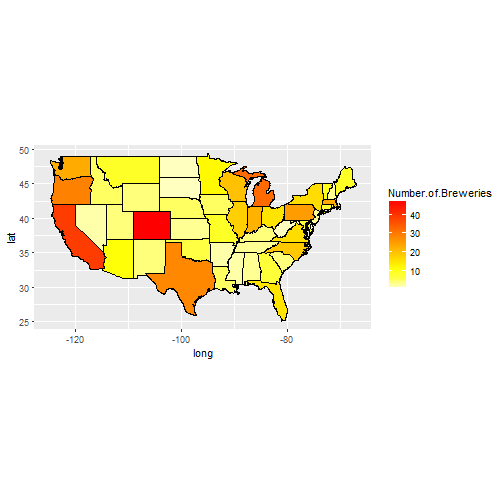
\includegraphics{Craft_Beer_Analysis_final_files/figure-latex/HeatMap-1.pdf}

\subsubsection{Question 2. Merge beer data with the breweries data.
Print the first 6 observations and the last six observations to check
the merged
file.}\label{question-2.-merge-beer-data-with-the-breweries-data.-print-the-first-6-observations-and-the-last-six-observations-to-check-the-merged-file.}

\begin{Shaded}
\begin{Highlighting}[]
\CommentTok{# There is one "Name" variable in each dataset. Change Variable names to distinguish between Beer and Brewery names}
\CommentTok{# Each dataset have different Brewery ID variable name. Change to Brewery_ID to match both datasets:}
\NormalTok{Breweries <-}\StringTok{ }\KeywordTok{rename}\NormalTok{(Breweries, }\DataTypeTok{Brewery_ID =} \NormalTok{Brew_ID, }\DataTypeTok{Brewery_Name =} \NormalTok{Name )}
\NormalTok{Beers <-}\StringTok{ }\KeywordTok{rename}\NormalTok{(Beers, }\DataTypeTok{Brewery_ID =} \NormalTok{Brewery_id, }\DataTypeTok{Beer_Name =} \NormalTok{Name)}

\CommentTok{#Order the data by Brewery and Beer_ID (not necessary because we are using the merge command, but useful anyway)}
\NormalTok{Beers <-}\StringTok{ }\NormalTok{Beers[}\KeywordTok{order}\NormalTok{(Beers$Brewery_ID,Beers$Beer_ID),]}

\CommentTok{#Check if the Brewery_ID values are the same in order to make sure they can be easily merged}
\KeywordTok{unique}\NormalTok{(Beers$Brewery_ID) ==}\StringTok{ }\KeywordTok{unique}\NormalTok{(Breweries$Brewery_ID)}
\end{Highlighting}
\end{Shaded}

\begin{verbatim}
##   [1] TRUE TRUE TRUE TRUE TRUE TRUE TRUE TRUE TRUE TRUE TRUE TRUE TRUE TRUE
##  [15] TRUE TRUE TRUE TRUE TRUE TRUE TRUE TRUE TRUE TRUE TRUE TRUE TRUE TRUE
##  [29] TRUE TRUE TRUE TRUE TRUE TRUE TRUE TRUE TRUE TRUE TRUE TRUE TRUE TRUE
##  [43] TRUE TRUE TRUE TRUE TRUE TRUE TRUE TRUE TRUE TRUE TRUE TRUE TRUE TRUE
##  [57] TRUE TRUE TRUE TRUE TRUE TRUE TRUE TRUE TRUE TRUE TRUE TRUE TRUE TRUE
##  [71] TRUE TRUE TRUE TRUE TRUE TRUE TRUE TRUE TRUE TRUE TRUE TRUE TRUE TRUE
##  [85] TRUE TRUE TRUE TRUE TRUE TRUE TRUE TRUE TRUE TRUE TRUE TRUE TRUE TRUE
##  [99] TRUE TRUE TRUE TRUE TRUE TRUE TRUE TRUE TRUE TRUE TRUE TRUE TRUE TRUE
## [113] TRUE TRUE TRUE TRUE TRUE TRUE TRUE TRUE TRUE TRUE TRUE TRUE TRUE TRUE
## [127] TRUE TRUE TRUE TRUE TRUE TRUE TRUE TRUE TRUE TRUE TRUE TRUE TRUE TRUE
## [141] TRUE TRUE TRUE TRUE TRUE TRUE TRUE TRUE TRUE TRUE TRUE TRUE TRUE TRUE
## [155] TRUE TRUE TRUE TRUE TRUE TRUE TRUE TRUE TRUE TRUE TRUE TRUE TRUE TRUE
## [169] TRUE TRUE TRUE TRUE TRUE TRUE TRUE TRUE TRUE TRUE TRUE TRUE TRUE TRUE
## [183] TRUE TRUE TRUE TRUE TRUE TRUE TRUE TRUE TRUE TRUE TRUE TRUE TRUE TRUE
## [197] TRUE TRUE TRUE TRUE TRUE TRUE TRUE TRUE TRUE TRUE TRUE TRUE TRUE TRUE
## [211] TRUE TRUE TRUE TRUE TRUE TRUE TRUE TRUE TRUE TRUE TRUE TRUE TRUE TRUE
## [225] TRUE TRUE TRUE TRUE TRUE TRUE TRUE TRUE TRUE TRUE TRUE TRUE TRUE TRUE
## [239] TRUE TRUE TRUE TRUE TRUE TRUE TRUE TRUE TRUE TRUE TRUE TRUE TRUE TRUE
## [253] TRUE TRUE TRUE TRUE TRUE TRUE TRUE TRUE TRUE TRUE TRUE TRUE TRUE TRUE
## [267] TRUE TRUE TRUE TRUE TRUE TRUE TRUE TRUE TRUE TRUE TRUE TRUE TRUE TRUE
## [281] TRUE TRUE TRUE TRUE TRUE TRUE TRUE TRUE TRUE TRUE TRUE TRUE TRUE TRUE
## [295] TRUE TRUE TRUE TRUE TRUE TRUE TRUE TRUE TRUE TRUE TRUE TRUE TRUE TRUE
## [309] TRUE TRUE TRUE TRUE TRUE TRUE TRUE TRUE TRUE TRUE TRUE TRUE TRUE TRUE
## [323] TRUE TRUE TRUE TRUE TRUE TRUE TRUE TRUE TRUE TRUE TRUE TRUE TRUE TRUE
## [337] TRUE TRUE TRUE TRUE TRUE TRUE TRUE TRUE TRUE TRUE TRUE TRUE TRUE TRUE
## [351] TRUE TRUE TRUE TRUE TRUE TRUE TRUE TRUE TRUE TRUE TRUE TRUE TRUE TRUE
## [365] TRUE TRUE TRUE TRUE TRUE TRUE TRUE TRUE TRUE TRUE TRUE TRUE TRUE TRUE
## [379] TRUE TRUE TRUE TRUE TRUE TRUE TRUE TRUE TRUE TRUE TRUE TRUE TRUE TRUE
## [393] TRUE TRUE TRUE TRUE TRUE TRUE TRUE TRUE TRUE TRUE TRUE TRUE TRUE TRUE
## [407] TRUE TRUE TRUE TRUE TRUE TRUE TRUE TRUE TRUE TRUE TRUE TRUE TRUE TRUE
## [421] TRUE TRUE TRUE TRUE TRUE TRUE TRUE TRUE TRUE TRUE TRUE TRUE TRUE TRUE
## [435] TRUE TRUE TRUE TRUE TRUE TRUE TRUE TRUE TRUE TRUE TRUE TRUE TRUE TRUE
## [449] TRUE TRUE TRUE TRUE TRUE TRUE TRUE TRUE TRUE TRUE TRUE TRUE TRUE TRUE
## [463] TRUE TRUE TRUE TRUE TRUE TRUE TRUE TRUE TRUE TRUE TRUE TRUE TRUE TRUE
## [477] TRUE TRUE TRUE TRUE TRUE TRUE TRUE TRUE TRUE TRUE TRUE TRUE TRUE TRUE
## [491] TRUE TRUE TRUE TRUE TRUE TRUE TRUE TRUE TRUE TRUE TRUE TRUE TRUE TRUE
## [505] TRUE TRUE TRUE TRUE TRUE TRUE TRUE TRUE TRUE TRUE TRUE TRUE TRUE TRUE
## [519] TRUE TRUE TRUE TRUE TRUE TRUE TRUE TRUE TRUE TRUE TRUE TRUE TRUE TRUE
## [533] TRUE TRUE TRUE TRUE TRUE TRUE TRUE TRUE TRUE TRUE TRUE TRUE TRUE TRUE
## [547] TRUE TRUE TRUE TRUE TRUE TRUE TRUE TRUE TRUE TRUE TRUE TRUE
\end{verbatim}

\begin{Shaded}
\begin{Highlighting}[]
\CommentTok{#Merge the datasets by Brewery_ID}
\NormalTok{MergedBeers <-}\StringTok{ }\KeywordTok{merge}\NormalTok{(}\DataTypeTok{x =} \NormalTok{Beers, }\DataTypeTok{y =} \NormalTok{Breweries, }\DataTypeTok{by =} \StringTok{"Brewery_ID"}\NormalTok{, }\DataTypeTok{all =} \OtherTok{TRUE}\NormalTok{)}
\KeywordTok{str}\NormalTok{(MergedBeers)}
\end{Highlighting}
\end{Shaded}

\begin{verbatim}
## 'data.frame':    2410 obs. of  10 variables:
##  $ Brewery_ID  : int  1 1 1 1 1 1 2 2 2 2 ...
##  $ Beer_Name   : Factor w/ 2305 levels "#001 Golden Amber Lager",..: 1525 1926 1640 2185 1258 802 2017 1570 1118 494 ...
##  $ Beer_ID     : int  2687 2688 2689 2690 2691 2692 2674 2675 2676 2677 ...
##  $ ABV         : num  0.056 0.06 0.06 0.048 0.049 0.045 0.05 0.06 0.065 0.051 ...
##  $ IBU         : int  47 25 38 19 26 50 20 65 NA 38 ...
##  $ Style       : Factor w/ 100 levels "","Abbey Single Ale",..: 57 22 83 48 77 16 48 16 26 90 ...
##  $ Ounces      : num  16 16 16 16 16 16 16 16 16 16 ...
##  $ Brewery_Name: Factor w/ 551 levels "10 Barrel Brewing Company",..: 355 355 355 355 355 355 12 12 12 12 ...
##  $ City        : Factor w/ 384 levels "Abingdon","Abita Springs",..: 228 228 228 228 228 228 200 200 200 200 ...
##  $ State       : Factor w/ 51 levels " AK"," AL"," AR",..: 24 24 24 24 24 24 18 18 18 18 ...
\end{verbatim}

\begin{Shaded}
\begin{Highlighting}[]
\NormalTok{### Print the first 6 observations and the last six observations to check the merged file.}
\KeywordTok{head}\NormalTok{(MergedBeers, }\DecValTok{6}\NormalTok{)}
\end{Highlighting}
\end{Shaded}

\begin{verbatim}
##   Brewery_ID     Beer_Name Beer_ID   ABV IBU
## 1          1   Parapet ESB    2687 0.056  47
## 2          1    Stronghold    2688 0.060  25
## 3          1       Pumpion    2689 0.060  38
## 4          1    Wall's End    2690 0.048  19
## 5          1 Maggie's Leap    2691 0.049  26
## 6          1  Get Together    2692 0.045  50
##                                 Style Ounces       Brewery_Name
## 1 Extra Special / Strong Bitter (ESB)     16 NorthGate Brewing 
## 2                     American Porter     16 NorthGate Brewing 
## 3                         Pumpkin Ale     16 NorthGate Brewing 
## 4                   English Brown Ale     16 NorthGate Brewing 
## 5                  Milk / Sweet Stout     16 NorthGate Brewing 
## 6                        American IPA     16 NorthGate Brewing 
##          City State
## 1 Minneapolis    MN
## 2 Minneapolis    MN
## 3 Minneapolis    MN
## 4 Minneapolis    MN
## 5 Minneapolis    MN
## 6 Minneapolis    MN
\end{verbatim}

\begin{Shaded}
\begin{Highlighting}[]
\KeywordTok{tail}\NormalTok{(MergedBeers, }\DecValTok{6}\NormalTok{)}
\end{Highlighting}
\end{Shaded}

\begin{verbatim}
##      Brewery_ID                 Beer_Name Beer_ID   ABV IBU
## 2405        556             Pilsner Ukiah      98 0.055  NA
## 2406        557         Porkslap Pale Ale      49 0.043  NA
## 2407        557         Moo Thunder Stout      50 0.049  NA
## 2408        557           Snapperhead IPA      51 0.068  NA
## 2409        557  Heinnieweisse Weissebier      52 0.049  NA
## 2410        558 Urban Wilderness Pale Ale      30 0.049  NA
##                        Style Ounces                  Brewery_Name
## 2405         German Pilsener     12         Ukiah Brewing Company
## 2406 American Pale Ale (APA)     12       Butternuts Beer and Ale
## 2407      Milk / Sweet Stout     12       Butternuts Beer and Ale
## 2408            American IPA     12       Butternuts Beer and Ale
## 2409              Hefeweizen     12       Butternuts Beer and Ale
## 2410        English Pale Ale     12 Sleeping Lady Brewing Company
##               City State
## 2405         Ukiah    CA
## 2406 Garrattsville    NY
## 2407 Garrattsville    NY
## 2408 Garrattsville    NY
## 2409 Garrattsville    NY
## 2410     Anchorage    AK
\end{verbatim}

\subsubsection{Question 3. Report the number of NA's in each
column.}\label{question-3.-report-the-number-of-nas-in-each-column.}

\begin{Shaded}
\begin{Highlighting}[]
\KeywordTok{sapply}\NormalTok{(MergedBeers, function(y) }\KeywordTok{sum}\NormalTok{(}\KeywordTok{is.na}\NormalTok{(y)))}
\end{Highlighting}
\end{Shaded}

\begin{verbatim}
##   Brewery_ID    Beer_Name      Beer_ID          ABV          IBU 
##            0            0            0           62         1005 
##        Style       Ounces Brewery_Name         City        State 
##            0            0            0            0            0
\end{verbatim}

Two columns have NA's: ABV has 62 and IBU has 1005, out of 2410 total
rows

\subsubsection{4. Compute the median alcohol content and international
bitterness unit for each state. Plot a bar chart to
compare.}\label{compute-the-median-alcohol-content-and-international-bitterness-unit-for-each-state.-plot-a-bar-chart-to-compare.}

\begin{Shaded}
\begin{Highlighting}[]
\NormalTok{## First do not select data with NA as their mean would be NA then so use split MergedBeers on state and}
\NormalTok{## get the mean of the split values with na.rm = TRUE}
\NormalTok{ABV.median <-}\StringTok{ }\KeywordTok{sapply}\NormalTok{(}\KeywordTok{split}\NormalTok{(MergedBeers, MergedBeers$State), function(y) }\KeywordTok{median}\NormalTok{(y$ABV, }\DataTypeTok{na.rm =} \OtherTok{TRUE}\NormalTok{))}

\NormalTok{IBU.median <-}\StringTok{ }\KeywordTok{sapply}\NormalTok{(}\KeywordTok{split}\NormalTok{(MergedBeers, MergedBeers$State), function(y) }\KeywordTok{median}\NormalTok{(y$IBU, }\DataTypeTok{na.rm =} \OtherTok{TRUE}\NormalTok{))}

\NormalTok{## Sort it in descending order}
\NormalTok{ABV.median.sort <-}\StringTok{ }\NormalTok{ABV.median[}\KeywordTok{order}\NormalTok{(-ABV.median)]}

\NormalTok{IBU.median.sort <-}\StringTok{ }\NormalTok{ABV.median[}\KeywordTok{order}\NormalTok{(-ABV.median)]}

\NormalTok{##plot a bar chart to compare}
\NormalTok{##Barplot of ABV value(s) vs State}
\KeywordTok{barplot}\NormalTok{(ABV.median.sort, }\DataTypeTok{main=}\StringTok{"ABV vs State"}\NormalTok{, }\DataTypeTok{xlab=}\StringTok{"State"}\NormalTok{, }\DataTypeTok{ylab=}\StringTok{"ABV Value(s)"}\NormalTok{, }\DataTypeTok{las=}\DecValTok{2}\NormalTok{)}
\end{Highlighting}
\end{Shaded}

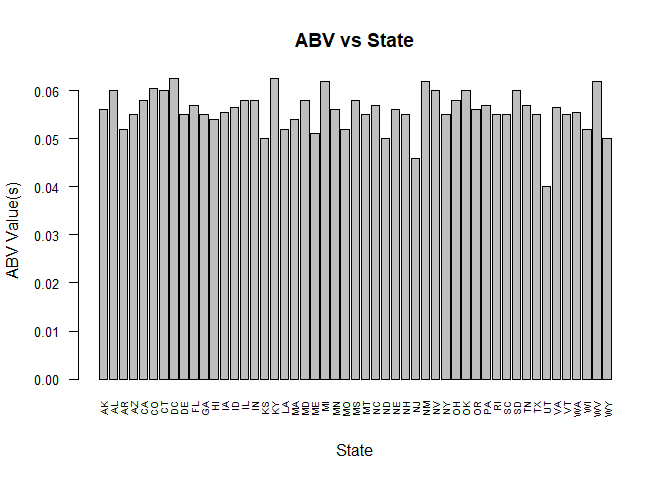
\includegraphics{Craft_Beer_Analysis_final_files/figure-latex/Question 4-1.pdf}

\begin{Shaded}
\begin{Highlighting}[]
\NormalTok{##Barplot of IBV value(s) vs State}
\KeywordTok{barplot}\NormalTok{(IBU.median.sort, }\DataTypeTok{main=}\StringTok{"IBV vs State"}\NormalTok{, }\DataTypeTok{xlab=}\StringTok{"State"}\NormalTok{, }\DataTypeTok{ylab=}\StringTok{"IBV Value(s)"}\NormalTok{, }\DataTypeTok{las=}\DecValTok{2}\NormalTok{)}
\end{Highlighting}
\end{Shaded}

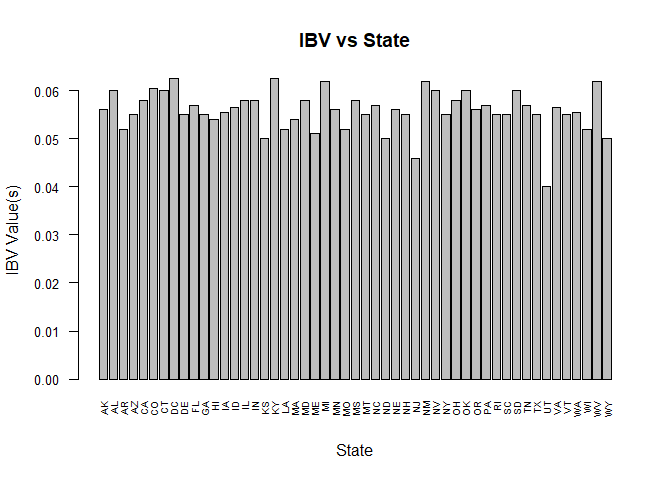
\includegraphics{Craft_Beer_Analysis_final_files/figure-latex/Question 4-2.pdf}

\subsubsection{5. Which state has the maximum alcoholic (ABV) beer?
Which state has the most bitter (IBU)
beer?}\label{which-state-has-the-maximum-alcoholic-abv-beer-which-state-has-the-most-bitter-ibu-beer}

\paragraph{State that has maximum alcoholic (ABV) beer is
CO.}\label{state-that-has-maximum-alcoholic-abv-beer-is-co.}

\paragraph{State that has most bitter (IBU) beer is
OR.}\label{state-that-has-most-bitter-ibu-beer-is-or.}

\begin{Shaded}
\begin{Highlighting}[]
\NormalTok{##State with maximum alcoholic (ABV) beer}
\KeywordTok{which}\NormalTok{(MergedBeers$ABV ==}\StringTok{ }\KeywordTok{max}\NormalTok{(MergedBeers$ABV, }\DataTypeTok{na.rm=}\OtherTok{TRUE}\NormalTok{))}
\end{Highlighting}
\end{Shaded}

\begin{verbatim}
## [1] 392
\end{verbatim}

\begin{Shaded}
\begin{Highlighting}[]
\NormalTok{MergedBeers$State[}\KeywordTok{which}\NormalTok{(MergedBeers$ABV ==}\StringTok{ }\KeywordTok{max}\NormalTok{(MergedBeers$ABV, }\DataTypeTok{na.rm=}\NormalTok{T))]}
\end{Highlighting}
\end{Shaded}

\begin{verbatim}
## [1]  CO
## 51 Levels:  AK  AL  AR  AZ  CA  CO  CT  DC  DE  FL  GA  HI  IA  ID ...  WY
\end{verbatim}

\begin{Shaded}
\begin{Highlighting}[]
\NormalTok{## State with maximum alcoholic (IBU) beer}
\NormalTok{MergedBeers$State[}\KeywordTok{which}\NormalTok{(MergedBeers$IBU ==}\StringTok{ }\KeywordTok{max}\NormalTok{(MergedBeers$IBU, }\DataTypeTok{na.rm=}\NormalTok{T))]}
\end{Highlighting}
\end{Shaded}

\begin{verbatim}
## [1]  OR
## 51 Levels:  AK  AL  AR  AZ  CA  CO  CT  DC  DE  FL  GA  HI  IA  ID ...  WY
\end{verbatim}

\subsubsection{6. Summary statistics for the ABV
variable.}\label{summary-statistics-for-the-abv-variable.}

\begin{Shaded}
\begin{Highlighting}[]
\NormalTok{##Sumary statistics for the ABV variable from the Beers dataset}
\KeywordTok{summary}\NormalTok{(Beers$ABV)}
\end{Highlighting}
\end{Shaded}

\begin{verbatim}
##    Min. 1st Qu.  Median    Mean 3rd Qu.    Max.    NA's 
## 0.00100 0.05000 0.05600 0.05977 0.06700 0.12800      62
\end{verbatim}

\begin{Shaded}
\begin{Highlighting}[]
\NormalTok{## Summary statistics for the ABV variable of the merged dataset}
\KeywordTok{summary}\NormalTok{(MergedBeers$ABV)}
\end{Highlighting}
\end{Shaded}

\begin{verbatim}
##    Min. 1st Qu.  Median    Mean 3rd Qu.    Max.    NA's 
## 0.00100 0.05000 0.05600 0.05977 0.06700 0.12800      62
\end{verbatim}

\subsubsection{7. Is there an apparent relationship between the
bitterness of the beer and its alcoholic content? Draw a scatter
plot.}\label{is-there-an-apparent-relationship-between-the-bitterness-of-the-beer-and-its-alcoholic-content-draw-a-scatter-plot.}

\paragraph{There seems to be an apparent relationship between the
bitterness of the beer and its alcoholic
content}\label{there-seems-to-be-an-apparent-relationship-between-the-bitterness-of-the-beer-and-its-alcoholic-content}

\begin{Shaded}
\begin{Highlighting}[]
\NormalTok{##Scatter plot between bitterness of beer and its alcoholic content}
\KeywordTok{plot}\NormalTok{(IBU~ABV, }\DataTypeTok{data=}\NormalTok{MergedBeers)}
\KeywordTok{abline}\NormalTok{(}\KeywordTok{lm}\NormalTok{(IBU~ABV, }\DataTypeTok{data=}\NormalTok{MergedBeers), }\DataTypeTok{col=}\StringTok{"red"}\NormalTok{)}
\end{Highlighting}
\end{Shaded}

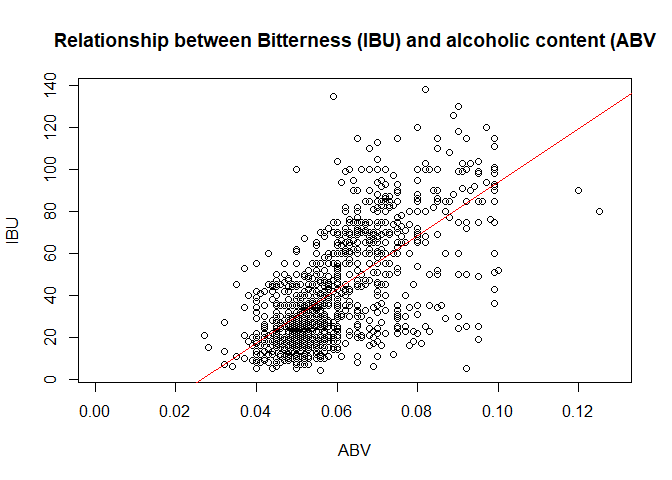
\includegraphics{Craft_Beer_Analysis_final_files/figure-latex/Question 7-1.pdf}

\subsubsection{Additional analysis}\label{additional-analysis}

\paragraph{Which styles of beer are more
popular?}\label{which-styles-of-beer-are-more-popular}

We'll create a barplot with the most popular beer styles:

\begin{Shaded}
\begin{Highlighting}[]
\CommentTok{# Create and sort the data}
\NormalTok{StyleFreqTable <-}\StringTok{ }\KeywordTok{as.data.frame}\NormalTok{(}\KeywordTok{table}\NormalTok{(Beers$Style))}
\NormalTok{StyleFreqTable <-}\StringTok{ }\NormalTok{StyleFreqTable[}\KeywordTok{order}\NormalTok{(-StyleFreqTable$Freq),]}
\KeywordTok{names}\NormalTok{(StyleFreqTable) <-}\StringTok{ }\KeywordTok{c}\NormalTok{(}\StringTok{"Style"}\NormalTok{, }\StringTok{"Frequency"}\NormalTok{)}
\CommentTok{# Plot the data}
\KeywordTok{ggplot}\NormalTok{(}\DataTypeTok{data =} \NormalTok{StyleFreqTable[}\DecValTok{1}\NormalTok{:}\DecValTok{20}\NormalTok{,], }\KeywordTok{aes}\NormalTok{(}\DataTypeTok{x =} \KeywordTok{reorder}\NormalTok{(Style, -Frequency), }\DataTypeTok{y =} \NormalTok{Frequency)) +}
\StringTok{  }\KeywordTok{geom_bar}\NormalTok{(}\KeywordTok{aes}\NormalTok{(}\DataTypeTok{fill =} \NormalTok{Style), }\DataTypeTok{stat =} \StringTok{"identity"}\NormalTok{, }\DataTypeTok{fill =} \StringTok{"lightblue"}\NormalTok{, }\DataTypeTok{color =} \StringTok{"black"}\NormalTok{) +}
\StringTok{  }\KeywordTok{labs}\NormalTok{(}\DataTypeTok{title =} \StringTok{"Most popular Styles of Beer"}\NormalTok{, }\DataTypeTok{x =} \StringTok{"Style of Beer"}\NormalTok{, }\DataTypeTok{y =} \StringTok{"Frequency"}\NormalTok{) +}
\StringTok{  }\KeywordTok{theme}\NormalTok{(}\DataTypeTok{axis.text.x =} \KeywordTok{element_text}\NormalTok{(}\DataTypeTok{angle =} \DecValTok{90}\NormalTok{, }\DataTypeTok{hjust =} \DecValTok{1}\NormalTok{))}
\end{Highlighting}
\end{Shaded}

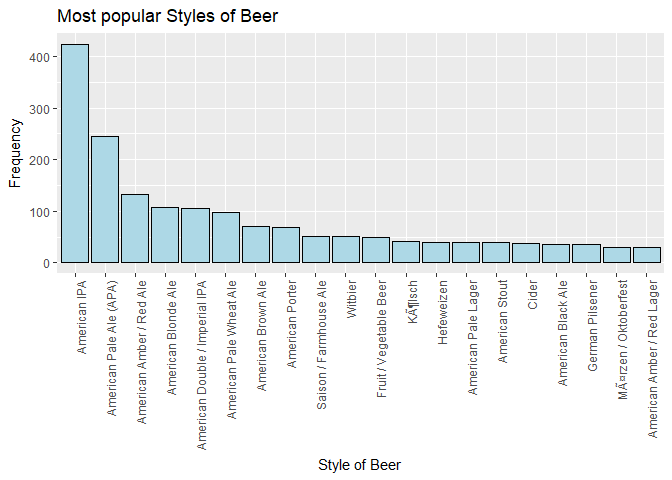
\includegraphics{Craft_Beer_Analysis_final_files/figure-latex/Bar plot of beer styles-1.pdf}

\paragraph{What words are more common in Beer
names?}\label{what-words-are-more-common-in-beer-names}

We'll create a word cloud to visualize which words are popular for beer
names

\begin{Shaded}
\begin{Highlighting}[]
\CommentTok{#Create file with the text of the Beer Names}
\NormalTok{text <-}\StringTok{ }\KeywordTok{as.character}\NormalTok{(Beers$Beer_Name)}
\NormalTok{docs <-}\StringTok{ }\KeywordTok{Corpus}\NormalTok{(}\KeywordTok{VectorSource}\NormalTok{(text))}
\NormalTok{toSpace <-}\StringTok{ }\KeywordTok{content_transformer}\NormalTok{(function (x , pattern ) }\KeywordTok{gsub}\NormalTok{(pattern, }\StringTok{" "}\NormalTok{, x))}
\NormalTok{docs <-}\StringTok{ }\KeywordTok{tm_map}\NormalTok{(docs, toSpace, }\StringTok{"/"}\NormalTok{)}

\CommentTok{# Convert the text to lower case}
\NormalTok{docs <-}\StringTok{ }\KeywordTok{tm_map}\NormalTok{(docs, }\KeywordTok{content_transformer}\NormalTok{(tolower))}
\CommentTok{# specify your stopwords as a character vector}
\NormalTok{docs <-}\StringTok{ }\KeywordTok{tm_map}\NormalTok{(docs, removeWords, }\KeywordTok{c}\NormalTok{(}\StringTok{"american"}\NormalTok{,}\StringTok{"#"}\NormalTok{, }\StringTok{"the"}\NormalTok{, }\StringTok{"ale"}\NormalTok{, }\StringTok{"ipa"}\NormalTok{, }\StringTok{"pale"}\NormalTok{, }\StringTok{"lager"}\NormalTok{))}
\CommentTok{# Remove numbers}
\NormalTok{docs <-}\StringTok{ }\KeywordTok{tm_map}\NormalTok{(docs, removeNumbers)}
\CommentTok{# Eliminate extra white spaces}
\NormalTok{docs <-}\StringTok{ }\KeywordTok{tm_map}\NormalTok{(docs, stripWhitespace)}

\NormalTok{dtm <-}\StringTok{ }\KeywordTok{TermDocumentMatrix}\NormalTok{(docs)}
\NormalTok{m <-}\StringTok{ }\KeywordTok{as.matrix}\NormalTok{(dtm)}
\NormalTok{v <-}\StringTok{ }\KeywordTok{sort}\NormalTok{(}\KeywordTok{rowSums}\NormalTok{(m),}\DataTypeTok{decreasing=}\OtherTok{TRUE}\NormalTok{)}
\NormalTok{d <-}\StringTok{ }\KeywordTok{data.frame}\NormalTok{(}\DataTypeTok{word =} \KeywordTok{names}\NormalTok{(v),}\DataTypeTok{freq=}\NormalTok{v)}
\CommentTok{#Create Word Cloud}
\KeywordTok{set.seed}\NormalTok{(}\DecValTok{1234}\NormalTok{)}
\KeywordTok{wordcloud}\NormalTok{(}\DataTypeTok{words =} \NormalTok{d$word, }\DataTypeTok{freq =} \NormalTok{d$freq, }\DataTypeTok{min.freq =} \DecValTok{10}\NormalTok{,}
          \DataTypeTok{max.words=}\DecValTok{200}\NormalTok{, }\DataTypeTok{random.order=}\OtherTok{FALSE}\NormalTok{, }\DataTypeTok{rot.per=}\FloatTok{0.35}\NormalTok{, }
          \DataTypeTok{colors=}\KeywordTok{brewer.pal}\NormalTok{(}\DecValTok{8}\NormalTok{, }\StringTok{"Dark2"}\NormalTok{))}
\end{Highlighting}
\end{Shaded}

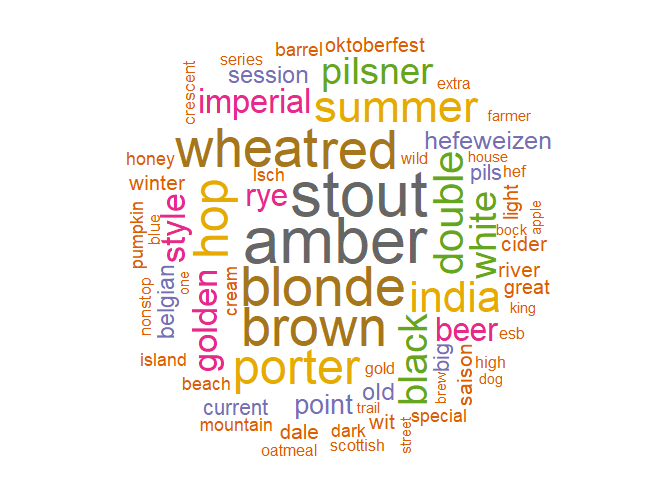
\includegraphics{Craft_Beer_Analysis_final_files/figure-latex/word cloud-1.pdf}
d \textless{}- d{[}order(-d\$freq),{]} \#\# \textbf{Section 4}
Conclusions

Pending


\end{document}
